\section{Code Generation}

Having completed semantic analysis, the compiler
can proceed to code generation.

\subsection{Passing on the \texttt{Environment} Tree}

Before, proceeding onto to the details of code generation it is
important to note that here is were all the upfront work that
was put into using \texttt{Environment} trees, pays off. This is
because there is no need to re-stablish the types of any of the
variables, at any scope.

\begin{lstlisting}[caption={Getting the global environment from
the \texttt{AnalysisVisitor} and passing it on for reordering
and code generation (runner/Runner.cpp).}]
std::unique_ptr<Environment> environment =
    mAnalyser.getEnvironment();

ReorderVisitor reorder{};

reorder.reorderAst(ast.get());

if (mParserDbg) {
    debugParsing(ast.get());
}

reorder.reorderEnvironment(environment.get());

GenVisitor gen{environment.get()};
\end{lstlisting}

\subsubsection{The \texttt{TypeVisitor} Class}

Having said that there is still the need to recompute the types
of expressions since the type of a composite expression e.g.
\texttt{2 + 3} cannot be stored in an \texttt{Environment}. To
handle this another visitor, this time called
\texttt{TypeVisitor} was created.

\begin{todo}
In the event that type checking/generation is completely
delegated to the \texttt{TypeVisitor}, future version of
compiler can drop usage of \texttt{Environment} trees in favour
of re-computing types as requested. Additionally, such a change
improves memory usage in exchange for time as described in
\ref{sss:memoryadvantage}.
\end{todo}

\begin{lstlisting}[caption={The \texttt{visit(FunctionCall *)}
method in the \texttt{TypeVisitor} class
(ir\_gen/TypeVisitor.cpp).}, label=lst:recomputefunctype]
void TypeVisitor::visit(core::FunctionCall *expr) {
    std::optional<Symbol> symbol{
        findSymbol(expr->identifier, mRefStack.getGlobal())
    };

    mReturn = symbol->as<FunctionSymbol>().returnType;

    expr->core::Expr::accept(this);
}
\end{lstlisting}

Currently, a \texttt{TypeVisitor} is given a \texttt{RefStack}
for \texttt{Environment} access and its main capability is
re-calculating the type of \textbf{already} type-checked
expressions (see \listref{recomputefunctype}).

\begin{marker}
Usage of a \texttt{TypeVisitor} on a non-type-checked expression
will at best crash and at worst still work, leading to undefined
behaviour.
\end{marker}

\subsection{Reordering}\label{sss:reordersec}

Due to the fact that the \texttt{PArDis} VM Simulator expects
all functions to be defined before the \texttt{.main} segment,
which in the case of \texttt{PArL} is everything not in a
function declaration, a solution needs to be devised to ensure
that this order requirement is satisfied.

A solution to this problem can be achieved by reordering the AST
and the \\ \texttt{Environment}s. Since function declarations can
only exist in global scope, moving them such that they are the
first statements, which are encountered, is a sufficient
modification to ensure code generation as required by the VM.

\begin{todo}
Currently the compiler has support for named scopes (see
backend/Environemnt.cpp, lines 25 and 34). With a specially
designed naming scheme to uniquely identify each scope, support
for nested functions can be enable by mangling function names
with scope names and lifting function declarations into global
scope.
\end{todo}

This approach required two visitors, named
\texttt{IsFunctionVisitor} and \\ \texttt{ReorderVisitor}, and a
function, \texttt{reorderEnvironment()} (the choice to embed it
into the \texttt{ReorderVisitor} was arbitrary).

The \texttt{IsFunctionVisitor} is quite self-explanatory, it is
a very simple visitor with an exposed method \texttt{check()},
which returns true only if a node is a function declaration.

\begin{lstlisting}[caption={The \texttt{reorder()} method in the
\texttt{ReorderVisitor} class (preprocess/ReorderVisitor.cpp).}]
void ReorderVisitor::reorder(
    std::vector<std::unique_ptr<core::Stmt>> &stmts
) {
    for (auto &stmt : stmts) {
        if (isFunction.check(stmt.get())) {
            mFuncQueue.push_back(std::move(stmt));
        } else {
            mStmtQueue.push_back(std::move(stmt));
        }
    }

    stmts.clear();

    for (auto &stmt : mFuncQueue) {
        stmts.push_back(std::move(stmt));
    }

    for (auto &stmt : mStmtQueue) {
        stmts.push_back(std::move(stmt));
    }

    reset();
}
\end{lstlisting}

The \texttt{ReorderVisitor} implements a method
\texttt{reorder()}, which is called only for program and block
nodes. The \texttt{reorder()} makes use of two queues. The first
queue keeps track of function declarations and the second queue
keeps track of everything else. The \texttt{reorder()} method
traverse the provided statement vector and enqueues statements
in there respective queues. Then the elements of the first queue
are dequeued back into the vector followed by  the elements of
second queue. Due to the usage of queues this essentially moves
all function declarations (in their original order) as the first
elements of the statements vector. The visitor is then accepted
by all the reordered statements.

\begin{note}
The visitor is accepted by the reordered statements, to cater
for the case when function declarations are also present in
other scopes not just the global scope. However, this is
currently not the case (see analysis/AnalysisVisitor.cpp, line
955).
\end{note}

\subsection{Function Declarations}

Due to the reordering described in \ref{sss:reordersec}, the
first nodes to be emitted are function declarations.

\begin{lstlisting}[escapechar=!, caption={The
\texttt{visit(FunctionDecl *)} method in the \texttt{GenVisitor}
class (ir\_gen/GenVisitor.cpp).}, label=lst:genfuncdecl]
void GenVisitor::visit(core::FunctionDecl *stmt) {
    Environment *nextEnv = mRefStack.peekNextEnv();

    size_t aritySize{0};

    for (auto &stmt : stmt->params) {
        aritySize +=
            !\colorbox{UMPaleRed}{mDeclCounter.count(stmt.get(),\
            nextEnv);}!
    }

    !\colorbox{UMPaleRed}{emit_line(".\{\}",\
    stmt->identifier);}!

    mRefStack.pushEnv(aritySize);

    for (auto &param : stmt->params) {
        !\colorbox{UMPaleRed}{param->accept(this);}!
    }

    stmt->block->accept(this);

    mRefStack.popEnv();
}
\end{lstlisting}

Again for code generation two more visitors apart from the
\texttt{TypeVisitor} were used. These are the
\texttt{GenVisitor} and the \texttt{VarDeclCountVisitor}.

\begin{lstlisting}[caption={The \texttt{visit(VariableDecl *)}
method in the \texttt{VarDeclCountVisitor} class
(ir\_gen/VarDeclCountVisitor.cpp)}, label=lst:vardeclcount]
void VarDeclCountVisitor::visit(core::VariableDecl *stmt) {
    std::optional<Symbol> symbol =
        mEnv->findSymbol(stmt->identifier);

    auto &variable = symbol->asRef<VariableSymbol>();

    mCount += variable.type.is<core::Array>()
                  ? variable.type.as<core::Array>().size
                  : 1;
}
\end{lstlisting}

The \texttt{GenVisitor} as its name suggest is the main visitor
which produces the VM instructions. The
\texttt{VarDeclCountVisitor} is an additional visitor which is
used to calculate the size of the memory required when opening a
frame on the VM.

\begin{note}\label{sss:framesizecalc}
Within the VM memory is implemented in the form a JavaScript
array. This means that there are no restrictions on how big a
single location is, for this reason there is no true standard
unit of size. However, it is implicitly assumed that the base
types: \texttt{bool}, \texttt{int}, \texttt{float} and
\texttt{color} all occupy single a unit. Hence, when calculating
the size of for example \texttt{int[4]} the
\texttt{VarDeclCountVisitor} returns $4$ (see
\listref{vardeclcount}).
\end{note}

\begin{lstlisting}[caption={The \texttt{emit\_line()} method in
the \texttt{GenVisitor} class (ir\_gen/GenVisitor.cpp).},
label=lst:emitline]
template <typename... T>
void emit_line(fmt::format_string<T...> fmt, T &&...args) {
    mCode.push_back(fmt::format(fmt, args...));
}
\end{lstlisting}

On the other hand, the main mechanism with which the
\texttt{GenVisitor} emits VM code is \texttt{emit\_line()}.
Again similar to \texttt{error()} and \texttt{warning()} (from
other visitors), \texttt{emit\_line()} wraps an fmtlib function
(see \listref{genfuncdecl} and \listref{emitline}).

In the context of function declarations the only significant
usage of \texttt{emit\_line()} is to output the identifier of
the function.

\subsection{Scopes, Variable (or Formal Parameter) Declarations
\& Variable Accesses}

\begin{lstlisting}[caption={The \texttt{visit(VariableDecl *)}
method in the \texttt{GenVisitor} class
(ir\_gen/GenVisitor.cpp).}, label=lst:formalparam]
void GenVisitor::visit(core::VariableDecl *stmt) {
    stmt->expr->accept(this);

    Environment *env = mRefStack.currentEnv();

    Environment *stoppingEnv = env;

    while (stoppingEnv->getType() !=
               Environment::Type::GLOBAL &&
           stoppingEnv->getType() !=
               Environment::Type::FUNCTION) {
        stoppingEnv = stoppingEnv->getEnclosing();
    }

    std::optional<Symbol> left{};

    for (;;) {
        left = env->findSymbol(stmt->identifier);

        if (left.has_value() || env == stoppingEnv)
            break;

        env = env->getEnclosing();
    }

    core::abort_if(
        !left.has_value(),
        "symbol is undefined"
    );

    size_t idx = env->getIdx();

    auto symbol = left->as<VariableSymbol>();

    if (symbol.type.is<core::Base>()) {
        env->incIdx();
    } else if (symbol.type.is<core::Array>()) {
        env->incIdx(symbol.type.as<core::Array>().size);
    } else {
        core::abort("unknown type");
    }

    // NOTE: make sure this is actually a reference.
    env->getSymbolAsRef(stmt->identifier)
        .asRef<VariableSymbol>()
        .idx = idx;

    if (symbol.type.is<core::Array>()) {
        emit_line(
            "push {}",
            symbol.type.as<core::Array>().size
        );
    }
    emit_line("push {}", idx);
    emit_line("push 0");
    if (symbol.type.is<core::Array>()) {
        emit_line("sta");
    } else {
        emit_line("st");
    }
}
\end{lstlisting}

Next, specific attention has to be given to variable
declarations and formal parameters. Referencing of variables or
formal parameters within the VM happens with the instruction
\mbox{\texttt{push [i:l]}} (for behaviour see
\figref{framesexp}). The key take-away from how this instruction
works is the fact that frames (which are actually just memory)
are accessed via an index (in the instruction \texttt{i}).

Hence, during code generation any reference to a variable or
formal parameter needs to happen through an index. This is why,
when defining a new variable or formal parameter, the internal
index of the current environment is copied into the variable or
formal parameter's  associated symbol. This facilitates
referencing a variable or formal parameter in the VM's
instructions (see \listref{formalparam} and
ir\_gen/GenVisitor.cpp, line 105).

Additionally, the index of the environment is incremented to the
next free position i.e. the next position a new variable or
formal parameter can be stored within the frame.

\begin{figure}[H]
\centering
\begin{mdframed}[backgroundcolor=OffWhite]
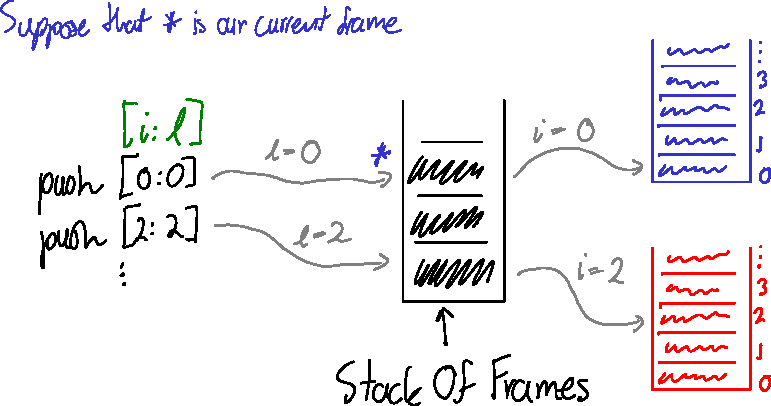
\includegraphics[width=\linewidth]{framesexp.pdf}
\end{mdframed}
\caption{A pictorial example of how the \mbox{\texttt{push
[i:l]}} operates.}
\label{fig:framesexp}
\end{figure}

\subsection{Properly Closing Scopes in Function Declarations}

A very important consideration when it comes to
function declarations is closing of scopes.

This is a problem of interest because functions should be
capable of returning anywhere within the body of a function even
if they are nested within multiple scopes.

\begin{lstlisting}[caption={A segment of the
\texttt{visit(Program *)} method in the \texttt{GenVisitor}
class (ir\_gen/GenVisitor.cpp).}, label=lst:framedepth]
...

emit_line("push {}", count);
emit_line("oframe");

mFrameDepth++;

...
\end{lstlisting}


\begin{lstlisting}[caption={The \texttt{visit(ReturnStmt *)}
method in the \texttt{GenVisitor} class
(ir\_gen/GenVisitor.cpp).}, label=lst:retstmt]
void GenVisitor::visit(core::ReturnStmt *stmt) {
    stmt->expr->accept(this);

    for (size_t i = 0; i < mFrameDepth; i++) {
        emit_line("cframe");
    }

    emit_line("ret");
}
\end{lstlisting}

To solve this issue, a variable \texttt{mFrameDepth} keeps track
of the number of frames open with the \texttt{oframe}
instruction, see \listref{framedepth}. When a return statement
node is reached the close frame instruction, \texttt{cframe}, is
emitted as many times as \\ \texttt{mFrameDepth} (see
\listref{retstmt}). This ensures that extra open frames are
closed before returning, allowing the VM to continue executing
the program normally.

\subsection{Assignments}

Similar, to when variables are first declared the store
(\texttt{st}) instruction is used for mutating the value in a
specified location. However, unlike variable declarations which
always define a level of $0$, assignments/mutations can occur on
variables defined in outer scopes. Hence, the level of variable
access needs to be calculated before being emitting \texttt{st}
and it necessary operands.

\begin{lstlisting}[caption={The \texttt{computeLevel()} method
in the \texttt{GenVisitor} class (ir\_gen/GenVisitor.cpp).},
label=lst:computelevel]
size_t GenVisitor::computeLevel(Environment *stoppingEnv) {
    size_t level = 0;

    Environment *env = mRefStack.currentEnv();

    while (stoppingEnv != env) {
        switch (env->getType()) {
            case Environment::Type::FOR:
            case Environment::Type::BLOCK:
                level++;
                break;
            case Environment::Type::FUNCTION:
                core::abort("unreachable");
                break;
            default:
                // noop
                break;
        }

        env = env->getEnclosing();
    }

    return level;
}
\end{lstlisting}

The basic idea for calculating the level of a variable is as
follows, copy the pointer to the \texttt{Environment} which
holds the variable then traverse from the current
\texttt{Environment} until the \texttt{Environment} with the
exact pointer as the \texttt{Environment} the variable was found
in is reached, all the while keeping track of the number of
scopes jumped through to reach said environment.

\begin{note}
Not, all \texttt{Environment}s contribute an open frame
(\texttt{oframe}), hence only certain types of scopes should be
counted as contributing to the number of levels. In the case of
\texttt{PArL} with its current restrictions, the only such
scopes are for-scopes and block-scopes (see
\listref{computelevel}).
\end{note}

\subsection{Expressions}

\subsubsection{Type Specific VM Code}

\begin{lstlisting}[caption={A segment of the
\texttt{visit(Binary *)} method in the \texttt{GenVisitor} class
(ir\_gen/GenVisitor.cpp).}, label=lst:overloadeddiv]
...
case core::Operation::DIV: {
    core::Primitive type = mType.getType(
        expr->right.get(),
        mRefStack.getGlobal(),
        mRefStack.currentEnv()
    );
    if (type == core::Primitive{core::Base::INT}) {
        expr->right->accept(this);
        expr->right->accept(this);
        expr->left->accept(this);
        emit_line("mod");
        expr->left->accept(this);
        emit_line("sub");
        emit_line("div");
    } else {
        expr->right->accept(this);
        expr->left->accept(this);
        emit_line("div");
    }
} break;
...
\end{lstlisting}

When it comes to expressions, due to the fact that operators
within the \texttt{PArL} language are overloaded some attention
to detail is required. The majority of the usage of
\texttt{TypeVisitor} is within expression nodes, specifically,
in places where behaviour is dependent on the operand's types.
For example in the case of division, the type of one of the
operands is computed (recall that semantic analysis guarantees
consistency of types, in the case of binary operations both the
left and right operands have the same type), then different
instructions are emitted depending on the returned type (see
\listref{overloadeddiv}).

\subsubsection{Function Calls}

\begin{lstlisting}[caption={The \texttt{visit(FunctionCall *)}
method in the \texttt{GenVisitor} class
(ir\_gen/GenVisitor.cpp).}, label=lst:funccall]
void GenVisitor::visit(core::FunctionCall *expr) {
    for (auto itr = expr->params.rbegin();
         itr != expr->params.rend();
         itr++) {
        (*itr)->accept(this);
    }

    size_t size{0};

    for (auto &param : expr->params) {
        core::Primitive paramType = mType.getType(
            param.get(),
            mRefStack.getGlobal(),
            mRefStack.currentEnv()
        );

        size += paramType.is<core::Array>()
                    ? paramType.as<core::Array>().size
                    : 1;
    }

    emit_line("push {}", size);
    emit_line("push .{}", expr->identifier);
    emit_line("call");
}
\end{lstlisting}

Functions calls are performed using the \texttt{call} VM
instruction. The most important aspect of function calls,
similar to scopes, is the calculation of the total size of the
parameters. This essentially determines how many operands will
be popped of off the operand stack and moved into the implicitly
created function frame. Additionally, it is important for all
the parameters of a function to be evaluated in reverse order
due to the fact that popping from the operand stack into the
function frame reverse the order of the parameters (see
\listref{funccall}).

\subsection{Branching}

Branching is somewhat challenging since at the jumping point the
compiler is unaware of how many instructions it might need to
jump. There are two possible solutions for this problem. The
first is to create a visitor which is capable of calculating the
number of instruction which a node expands to. The second makes
use of a placeholder instruction that is then changed after the
rest of the associated instructions are generated.

Previous iterations of the \texttt{PArL} compiler used the first
approach however, the first approach is quite unmaintainable
since changes in other areas of the code generation would
require changes in the visitor which computes the number of
instructions. Hence, the compiler was changed to adopt the
second approach.

\texttt{PArL} has only three node types which branch, if-else
statements, for-loops and while-loops.

\begin{lstlisting}[caption={The \texttt{visit(WhileStmt *)}
method in the \texttt{GenVisitor} class
(ir\_gen/GenVisitor.cpp).}, label=lst:whilestmtgen]
void GenVisitor::visit(core::WhileStmt *stmt) {
    mRefStack.pushEnv();

    size_t condOffset = PC();

    stmt->cond->accept(this);

    emit_line("not");

    size_t patchOffset = PC();

    emit_line("push #PC+{{}}");
    emit_line("cjmp");

    stmt->block->accept(this);

    emit_line("push #PC-{}", PC() - condOffset);
    emit_line("jmp");

    mCode[patchOffset] =
        fmt::format(mCode[patchOffset], PC() - patchOffset);

    mRefStack.popEnv();
}
\end{lstlisting}

Both for-loops and while-loops branch in the same manner.
Patching the relevant instructions for branching in for- and
while-loops works as follows (additionally, see
\listref{whilestmtgen}):

\begin{enumerate}
    \item The location of the instruction which starts the
        condition is stored (in this case in
        \texttt{condOffset});
    \item the location of the `\texttt{push \#PC+\{\}}'
        instruction used for \texttt{cjmp} is stored (in this
        case in \texttt{patchOffset});
    \item then the block associated with the for- or while-loop
        accepts the \texttt{GenVisitor}, emitting further
        instructions;
    \item the offset required to jump back to the
        start of the condition instructions is calculated and
        used with a \texttt{jmp} instruction;
    \item and finally, the `\texttt{push \#PC+\{\}}' instruction
        at \texttt{patchOffset} is patched with the appropriate
        offset to jump clear all of the for- or while- loop
        instructions.
\end{enumerate}

\begin{lstlisting}[caption={The \texttt{visit(IfStmt *)} method
in the \texttt{GenVisitor} class (ir\_gen/GenVisitor.cpp).},
label=lst:ifstmtgen]
void GenVisitor::visit(core::IfStmt *stmt) {
    if (stmt->elseBlock) {
        mRefStack.pushEnv();

        stmt->cond->accept(this);

        emit_line("not");

        size_t ifPatchOffset = PC();

        emit_line("push #PC+{{}}");
        emit_line("cjmp");

        stmt->thenBlock->accept(this);

        mRefStack.popEnv();

        mRefStack.pushEnv();

        size_t elsePatchOffset = PC();

        emit_line("push #PC+{{}}");
        emit_line("jmp");

        mCode[ifPatchOffset] = fmt::format(
            mCode[ifPatchOffset],
            PC() - ifPatchOffset
        );

        stmt->elseBlock->accept(this);

        mCode[elsePatchOffset] = fmt::format(
            mCode[elsePatchOffset],
            PC() - elsePatchOffset
        );

        mRefStack.popEnv();
    } else {
        mRefStack.pushEnv();

        stmt->cond->accept(this);

        emit_line("not");

        size_t patchOffset = PC();

        emit_line("push #PC+{{}}");
        emit_line("cjmp");

        stmt->thenBlock->accept(this);

        mCode[patchOffset] = fmt::format(
            mCode[patchOffset],
            PC() - patchOffset
        );

        mRefStack.popEnv();
    }
}
\end{lstlisting}

The other form of branching, if-else statements, is a bit more
involved. This is because there are two cases which need
consideration: when only an \texttt{if} is present and when both
an \texttt{if} and an \texttt{else} are present. Nevertheless,
the basic principal is the same, offsets into the code are used
and specific lines are patched after (see \listref{ifstmtgen}).
